\documentclass[12pt]{article}
    \usepackage{psfrag}
    \usepackage{graphicx}
    \usepackage{xcolor}
    \pagestyle{empty}
  
    % You can run this by typing the following commands:
    %    latex vdp.tex
    %    dvips -o vdp.ps vdp.dvi
  
    \begin{document}
  
    % The syntax of the "psfrag" command is:
    %    \psfrag{tag}[<posn>][<psposn>][<scale>][<rot>]{replacement}
    % See the file pfgguide.ps for full documentation.
  
    \begin{figure}
      \psfrag{X}[B][B][1][0]{$x$}
      \psfrag{Y}[Bl][Bl][1][0]{$y$}
      \psfrag{YPSI}[Bl][Bc][1][0]{\color{blue} $x(1-v)=y$}
      \psfrag{XPHI}[B][c][1][0]{\color{brown} $ px =  y^3 + s y^2  - ry $}
      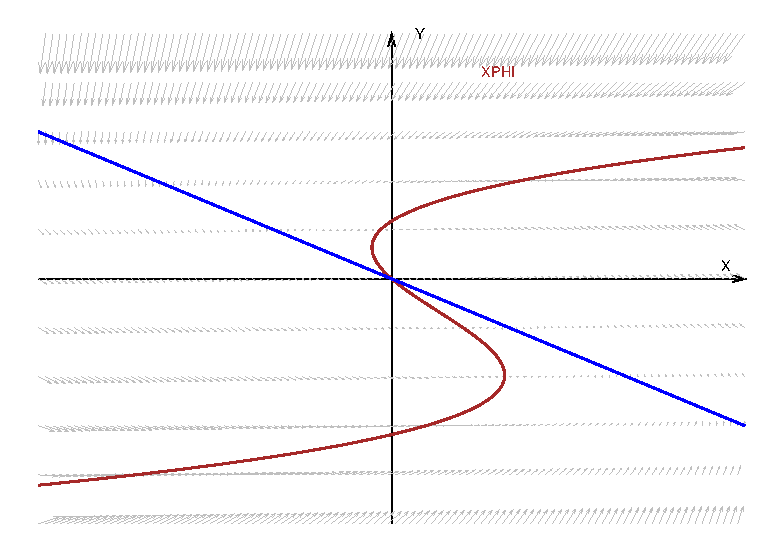
\includegraphics{saltzman.eps}
    \end{figure}
  
    \end{document}


